%%%%%%%%%%%%%%%%%%%%%%%%%%%%%%%%%%% CABECALHO %%%%%%%%%%%%%%%%%%%%%%%%%%%%%%%%%%%
\documentclass[a4paper]{abnt}

\usepackage[utf8]{inputenc}
\usepackage{csquotes}
\usepackage[brazil]{babel}
\usepackage[T1]{fontenc}
\usepackage[all,defaultlines=2]{nowidow}
\usepackage[multiple]{footmisc}
\usepackage{xcolor,graphicx}
\usepackage[backend=bibtex,backref=true]{biblatex}
\usepackage[colorlinks=true,urlcolor=blue,linkcolor=black,citecolor=red]{hyperref}

\bibliography{projeto}

\author{Igor~Santos}
\title{Projeto~de~TCC - Insert~Coin}

\makeindex
\begin{document}
\maketitle

%%%%%%%%%%%%%%%%%%%%%%%%%%%%%%%%%%%%% INICIO %%%%%%%%%%%%%%%%%%%%%%%%%%%%%%%%%%%%%

\tableofcontents

\chapter{Proposta do Projeto de TCC}

O projeto a ser desenvolvido é um Sistema Pessoal de Planejamento Financeiro, ou de Controle Orçamentário, ou ainda, um Administrador de
Finanças. Seu objetivo é transformar a organização financeira de uma pessoa ou de uma residência, facilitando o manuseio e controle de entrada e saída do dinheiro e das contas bancárias, bem como do cartão de crédito – neste, alterando a forma como o usuário comumente vê o ``plástico''.

Em verdade, o principal diferencial do produto em relação à concorrência atual no mercado será o controle de cartões de crédito. O brasileiro tem o costume de considerar o cartão como um ``gasto'', uma despesa que atrapalha o bom andamento do orçamento familiar, sendo assim um ``mal necessário'' devido aos seus benefícios no adiamento de compras.

O objetivo do \textbf{Insert Coin} nesse sentido é auxiliar o usuário no entendimento dos seus cartões de crédito, e integrá-los ao seu fluxo de caixa normal. Tal fluxo é comumente baseado na entrada de poucas fontes de renda (de alto volume), e a saída em diversas despesas mensais (de volume menor). O cartão de crédito, por ser um concentrador de despesas que adia o pagamento de diversos eventos para um único dia, tende mais confundir do que a ajudar. O usuário precisa compreender bem a dinâmica dos dias de fechamento e de abertura de nova fatura, do ``melhor dia para compra'', o dia do vencimento e quais são os valores possíveis de pagamento – e quais as consequências de não pagar a fatura por completo. Além disso, o lançamento de despesas ocorre com diversos dias de diferença entre o evento e seu aparecimento na fatura parcial. Tudo isso vai muito além do fluxo simples de sua conta-corrente e seu cartão de débito, que consiste em receber o salário do mês, e lançamentos instantâneos do uso do cartão de débito.

%%%%%%%%%%%%%%%%%%%%%%%%%%%%%%%%%%%%%%%%%%%%%%%%%%%%%%%%%%%%%%%%%%%%%%%%%%%%%%%%%%%%%%%%%
\section{O Projeto}

Inicialmente chamado de \textbf{Insert Coin}, ele é principalmente um sistema baseado no lançamento de entradas e saídas de uma ou mais contas de finanças. Ele se assemelha à organização de um Livro-Caixa empresarial, onde o usuário marcará todos os valores recebidos e gastos de uma determinada conta. 

Atualmente existem diversos sistemas no mercado, tanto web quanto móvel, que atendem a esse tipo de usuário, auxiliando na visualização e controle das despesas mensais. Boa parte deles tem o mesmo princípio, inclusive. Portanto, se considerarmos somente esta \emph{feature}, o sistema será pouco diferente do que já existe no mercado e, por exemplo, não incentivará a migração dos usuários de concorrentes para o nosso projeto. Para remediar isso tentaremos inovar na interface e na facilidade de entrada de dados, que é um dos grandes obstáculos para a introdução deste tipo de sistema na rotina do usuário.

Por outro lado, somente um dos sistemas encontrados tenta suprir as peculiaridades do mercado de cartões de crédito nacional, de forma muito vaga e primariamente informativa. O método a ser utilizado aqui é bem mais ativo: ele auxilia o usuário a entender como o cartão de crédito afeta seu fluxo de caixa e insere, como despesas comuns, os eventos nos quais o cartão foi utilizado. O objetivo é evitar a segregação comum que o brasileiro faz em considerar o cartão de crédito com uma mais uma conta/boleto a pagar, como é a eletricidade ou a água da casa. No cartão são feitos gastos assim como ocorrem na conta de débito: lazer, vestuário, transporte, educação, etc. Portanto, porque devemos pensar em ``reduzir os gastos do cartão'' ao invés de ``reduzir os gastos mensais''?

Trabalhando de forma unificada será mais fácil para o usuário compreender o destino do dinheiro daquele mês. Também será possível começar a planejar e organizar metas de redução dos gastos, ou objetivos de economia de forma eficiente e focada. Essa unificação ocorrerá a partir da visualização das despesas daquele mês com relação às entradas; o usuário não precisará se perder em filtros de datas distintos entre a conta-corrente e o cartão de crédito -- que naturalmente possuem fluxos temporais diferenciados. O sistema também evitará a dúvida comum ``será que já posso usar o cartão de crédito?'', auxiliando o usuário a entender as datas importantes de seus cartões, e as inserindo na rotina que ele já conhece e compreende -- a de sua conta corrente e salário.

O que mais cria dúvidas no cartão de crédito é que sua fatura é finalizada cerca de 10 dias antes do dia de pagamento. Aquele período é quando o usuário não está certo de onde as despesas se encaixam melhor: se no mês atual ou no seguinte. Essa confusão se acentua pois as datas da fatura dificilmente encapsulam o período de mês com o qual o usuário está financeiramente acostumado: seu fluxo mensal de entrada do salário. Se ele decide colocar o vencimento do cartão para uma data próxima de seu salário, o fechamento da fatura fica distante do final do mês; se decide fechar a fatura no final do mês, o pagamento fica distante das outras contas que ele comumente paga. E muitas vezes algumas despesas de uma determinada só serão pagas dali a dois meses, o que gera confusão e certa negligência na hora de conferir a origem dos gastos.

A proposta é coletar as datas importantes do cartão e orientar o usuário para que, sempre que possível, a fatura seja paga em cheio no dia do vencimento (em débito automático, por exemplo). Esta é, de acordo com os especialistas da área, a melhor forma de conviver com o cartão, pois não gera juros adicionais em cima do que não foi pago. A partir daí, o usuário terá configurada sua conta-corrente do sistema para que as despesas que ocorrerem no cartão de crédito sejam visualizadas simultaneamente às da conta, no período que corresponda ao pagamento da fatura. Conforme vão surgindo novas despesas no cartão de crédito, o usuário poderá visualizar diretamente seu o impacto no orçamento dos meses seguintes. Também será possível entender de forma prática a fatura do cartão do mês em visualização, juntamente com as contas a serem pagas e as despesas comuns em débito -- afinal de contas, é na conta-corrente que a ação financeira acontece.

%%%%%%%%%%%%%%%%%%%%%%%%%%%%%%%%%%%%%%%%%%%%%%%%%%%%%%%%%%%%%%%%%%%%%%%%%%%%%%%%%%%%%%%%%
\section{Método de Trabalho}
O desenvolvimento do sistema será gerido a partir da área de \emph{Issues} do \textbf{Github}. Lá é possível criar tarefas, categorizar (a partir de \emph{tags}), delegar e ordenar temporalmente. O andamento do projeto será acompanhado a partir de \emph{milestones} configurados no mesmo subsistema, todos com claras datas de finalização.

O \textbf{Github}, além de possuir um subsistema de tarefas, serve principalmente para armazenar na \emph{cloud} um servidor centralizado de \emph{git}. Dessa forma temos automaticamente um sistema eficiente de backup do código do sistema. Ele também participa do ambiente auxiliando a entender o histórico de desenvolvimento no decorrer do tempo; o \emph{git} armazena todas as alterações de código que forem feitas, o que nos ajuda a analisar nossa produtividade e facilmente encontrar os responsáveis por partes do sistema -- útil, por exemplo, quando ocorrer um \emph{bug} inesperado e que precisa ser rapidamente corrigido.

Por fim, para organizar o fluxo de código, será utilizado o \emph{GitFlow}\cite{gitflow} uma metodologia de versionamento que organiza as \emph{tags} de um repositório de forma lógica. A organização precisa desse sistema nos permite criar um fluxo contínuo de \emph{deploys}; podemos configurar nossos servidores de produção para \emph{escutarem} a \emph{tag master} e sempre que houver novos \emph{commits}, eles podem importar a nova versão - isso é feito a partir de \emph{git hooks}, ou automaticamente por alguns sistemas de \emph{PaaS}.

\begin{figure}
	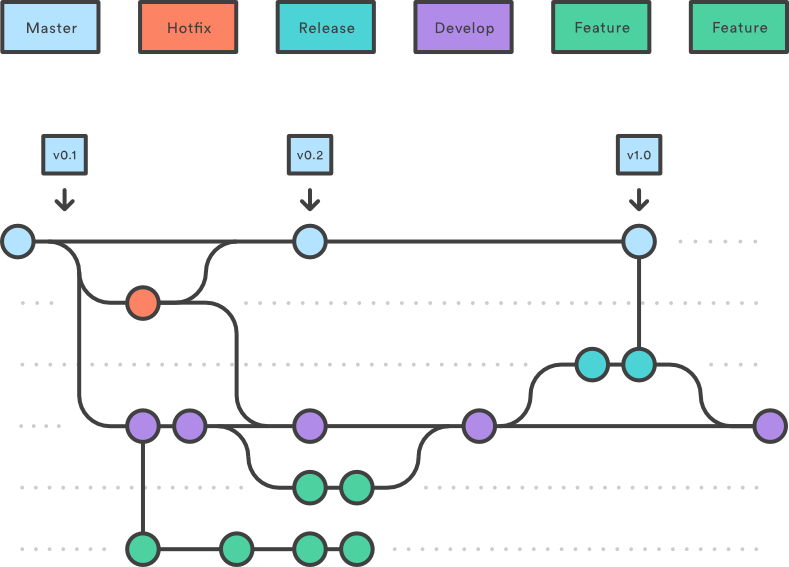
\includegraphics[scale=0.65]{img/gitflow.png}
	\caption{Exemplo de como \emph{GitFlow} funciona, exibindo os diversos \emph{branches} da metodologia.}
\end{figure}

%%%%%%%%%%%%%%%%%%%%%%%%%%%%%%%%%%%%%%%%%%%%%%%%%%%%%%%%%%%%%%%%%%%%%%%%%%%%%%%%%%%%%%%%%
\section{Previsão de Alocação de Recursos}

\subsection*{Recursos Humanos}
\begin{itemize}
	\item 1 Analista de Sistemas Sênior;
	\item 1 Designer multi-plataforma (\textit{web} e móvel);\footnotemark
	\item 1 Analista de marketing \emph{freelancer} (para o marketing inicial do produto; futuramente, integrará a equipe permanente).
\end{itemize}

\subsection*{Recursos Materiais}
\begin{itemize}
	\item Instâncias no \emph{Heroku} (é possível começar com pouco e expandir facilmente no futuro\cite{heroku}) com as seguintes configurações / add-ons:
	\begin{itemize}
		\item \emph{Dynos} (máquinas que processam \emph{requests} web) com \textbf{PHP 5.5}
		\item Servidor \textbf{PostgreSQL}, também facilmente escalável e seguro\cite{heroku-pgsql}
		\item Servidor de \emph{Memcache} \textbf{MemCachier} para caches temporários de aplicação
		\item \textbf{Mandrill by MailChimp} para envio de e-mails de lembretes
		\item \textbf{NewRelic} para monitoria da performance da aplicação e do banco de dados
		\item \textbf{Rollbar} para monitoria de erros nas aplicações
	\end{itemize}
\end{itemize}

%%%%%%%%%%%%%%%%%%%%%%%%%%%%%%%%%%%%%%%%%%%%%%%%%%%%%%%%%%%%%%%%%%%%%%%%%%%%%%%%%%%%%%%%%
\section{Cronograma de Trabalho}
\emph{Diagrama de Gantt.}

%%%%%%%%%%%%%%%%%%%%%%%%%%%%%%%%%%%%%%%%%%%%%%%%%%%%%%%%%%%%%%%%%%%%%%%%%%%%%%%%%%%%%%%%%
\chapter{A Empresa e o Negócio}
O objetivo do projeto é entrar num mercado já saturado de aplicativos similares com uma lista de diferenciais para atrair os consumidores que ainda não utilizam sistemas automatizados de gestão financeira ou se sentem insatisfeitos com as soluções que usam atualmente. Para isso, a equipe de desenvolvimento focará numa usabilidade simples e no menor atrito possível para entrada de novos lançamentos. E, por outro lado, o diferencial em funcionalidades terá como carro-chefe o tratamento do cartão de crédito de forma diferenciada das contas corrente e poupança, como nenhum aplicativo do mercado faz atualmente.

Todos os responsáveis pelo projeto tem larga experiência prática em diversos métodos de organização financeira e são usuários de diferentes sistemas do mercado. Portanto, todos são hábeis de opinar e desenvolver o projeto da melhor forma possível, com boas sugestões de funcionalidades e ao mesmo tempo evitando os erros (de acordo com nosso ponto de vista) já cometidos pela concorrência.

O sistema funcionará no modo \textit{freemium}, onde os usuários terão acesso a um grupo limitado de funcionalidades e precisarão pagar mensalmente caso desejem utilizar as funções avançadas. A lista final do que será de uso gratuito e do que será pago só será de fato conhecida quando o escopo do projeto for fechado; no entanto, segue um exemplo de algumas funcionalidades mais complexas e que fazem sentido entrar na lista \textit{premium}:
\begin{itemize}
	\item Gráficos e análises financeiras sobre os gastos mensais e anuais
	\item Ter mais de duas contas (sendo uma corrente e uma poupança\footnote{Isso caracterizaria um usuário avançado, visto que o caso mais comum é o brasileiro ter uma conta-corrente onde recebe seu pagamento (ou uma conta-salário e uma corrente), e talvez uma poupança onde ele guarda suas economias, e diversos cartões de crédito.})
	\item A possibilidade de planejar o pagamento parcial de uma fatura de cartão de crédito
	\item Uso do aplicativo móvel em modo offline, permitindo sincronia de dados quando o aparelho entrar numa conexão \textit{WiFi}
	\item Integração entre mais de um usuário numa mesma conta -- por exemplo, um casal usando o mesmo sistema a partir de dois \textit{logins} diferentes
\end{itemize}
 
%%%%%%%%%%%%%%%%%%%%%%%%%%%%%%%%%%%%%%%%%%%%%%%%%%%%%%%%%%%%%%%%%%%%%%%%%%%%%%%%%%%%%%%%%
\section{Histórico}
A empresa responsável pelo \textbf{Insert Coin} foi criada especialmente para o projeto, a partir da sintonia de ideias entre o Analista e o Designer a cargo. A ideia surgiu quando o Analista se sentia insatisfeito com o sistema de gestão que utilizava e não conseguiu encontrar substituto eficaz no mercado. O que mais lhe incomodava era não ser fácil controlar os gastos em cartão de crédito, pois as aplicações disponíveis só possuíam a distinção entre múltiplas ``contas'', e o ciclo de vida de uma fatura acabava por ficar misturado com o fluxo de caixa da conta-corrente, por exemplo. A ideia foi fomentada aos poucos e então surgiu a oportunidade de, junto ao seu colega de graduação, iniciar a estruturação e o desenvolvimento do projeto.

%%%%%%%%%%%%%%%%%%%%%%%%%%%%%%%%%%%%%%%%%%%%%%%%%%%%%%%%%%%%%%%%%%%%%%%%%%%%%%%%%%%%%%%%%
\section{Mercado Consumidor}
O público-alvo do projeto tem uma ou mais de cada uma das seguintes características:
\begin{enumerate}
	\item Em relação às suas finanças:
		\begin{itemize}
			\item Nunca se informou sobre educação financeira antes, mas começou a se interessar sobre o assunto;
			\item Já tem um certo nível de organização financeira, mas ela é falha ou rudimentar;
			\item Tem suas planilhas eletrônicas financeiras, mas são complexas de usar e engessadas;
			\item Encontra problemas de se manter no azul, e está em busca de de soluções para sua falta de controle;
		\end{itemize}
	\item Em relação à tecnologia:
		\begin{itemize}
			\item Possui um smartphone e tem um uso aceitável do mesmo, mas não usa o computador com frequência;
			\item Possui ou não um smartphone e se sente confortável navegando na Internet;
			\item Possui ou não um smartphone e utiliza planilhas eletrônicas para controlar suas finanças;
		\end{itemize}
\end{enumerate}

Ou seja, nosso principal mercado consumidor tem algum contato com tecnologia e se sente confortável a usá-la, seja no computador ou num dispositivo móvel, e tem algum interesse em educação e organização financeira, seja por dificuldades anteriores ou por puro interesse pessoal.

%%%%%%%%%%%%%%%%%%%%%%%%%%%%%%%%%%%%%%%%%%%%%%%%%%%%%%%%%%%%%%%%%%%%%%%%%%%%%%%%%%%%%%%%%
\section{Concorrência}
\emph{Falar brevemente sobre as empresas dos produtos concorrentes}

%%%%%%%%%%%%%%%%%%%%%%%%%%%%%%%%%%%%%%%%%%%%%%%%%%%%%%%%%%%%%%%%%%%%%%%%%%%%%%%%%%%%%%%%%
\section{Premissas e Restrições ao Projeto}
\emph{Explicar as ideias basicas e features essenciais, e o que nao sera possivel fazer no momento ou fica fora do escopo ideal do projeto.}

%%%%%%%%%%%%%%%%%%%%%%%%%%%%%%%%%%%%%%%%%%%%%%%%%%%%%%%%%%%%%%%%%%%%%%%%%%%%%%%%%%%%%%%%%
\chapter{Os Sistemas Atuais}

%%%%%%%%%%%%%%%%%%%%%%%%%%%%%%%%%%%%%%%%%%%%%%%%%%%%%%%%%%%%%%%%%%%%%%%%%%%%%%%%%%%%%%%%%
\section{Principais Concorrentes}
\emph{Descrever os principais sistemas do mercado atual, como Granatum, Mint, Monefy, Yupee, etc}

%%%%%%%%%%%%%%%%%%%%%%%%%%%%%%%%%%%%%%%%%%%%%%%%%%%%%%%%%%%%%%%%%%%%%%%%%%%%%%%%%%%%%%%%%
\section{Outros Sistemas}
\emph{Explicar sobre outras formas de organizacao financeira e suas vantagens e desvantagens, como o uso de um caderno manual, ou planilhas eletronicas.}

%%%%%%%%%%%%%%%%%%%%%%%%%%%%%%%%%%%%%%%%%%%%%%%%%%%%%%%%%%%%%%%%%%%%%%%%%%%%%%%%%%%%%%%%%
\section{Motivação para o Novo Sistema}
\emph{Porque o nosso sistema seria melhor que os atuais?}

%%%%%%%%%%%%%%%%%%%%%%%%%%%%%%%%%%%%%%%%%%%%%%%%%%%%%%%%%%%%%%%%%%%%%%%%%%%%%%%%%%%%%%%%%
\subsection{Problemas dos Sistemas Atuais}
\emph{Desvantagens da concorrencia}

%%%%%%%%%%%%%%%%%%%%%%%%%%%%%%%%%%%%%%%%%%%%%%%%%%%%%%%%%%%%%%%%%%%%%%%%%%%%%%%%%%%%%%%%%
\subsection{Situação Desejada}
\emph{Objetivos do nosso sistema}

%%%%%%%%%%%%%%%%%%%%%%%%%%%%%%%%%%%%%%%%%%%%%%%%%%%%%%%%%%%%%%%%%%%%%%%%%%%%%%%%%%%%%%%%%
\chapter{O Sistema Proposto}

%%%%%%%%%%%%%%%%%%%%%%%%%%%%%%%%%%%%%%%%%%%%%%%%%%%%%%%%%%%%%%%%%%%%%%%%%%%%%%%%%%%%%%%%%
\section{Requisitos do Sistema}

%%%%%%%%%%%%%%%%%%%%%%%%%%%%%%%%%%%%%%%%%%%%%%%%%%%%%%%%%%%%%%%%%%%%%%%%%%%%%%%%%%%%%%%%%
\section{Casos de Uso}

%%%%%%%%%%%%%%%%%%%%%%%%%%%%%%%%%%%%%%%%%%%%%%%%%%%%%%%%%%%%%%%%%%%%%%%%%%%%%%%%%%%%%%%%%
\subsection{Diagramas}

%%%%%%%%%%%%%%%%%%%%%%%%%%%%%%%%%%%%%%%%%%%%%%%%%%%%%%%%%%%%%%%%%%%%%%%%%%%%%%%%%%%%%%%%%
\subsection{Especificações}

%%%%%%%%%%%%%%%%%%%%%%%%%%%%%%%%%%%%%%%%%%%%%%%%%%%%%%%%%%%%%%%%%%%%%%%%%%%%%%%%%%%%%%%%%
\section{Diagrama Geral de Fluxo de Comunicação (Topologia?)}
\emph{Indicar aqui o fluxo de comunicacao entre o servidor REST e os mecanismos de cache da rede e dos aplicativos web e mobile.}

%%%%%%%%%%%%%%%%%%%%%%%%%%%%%%%%%%%%%%%%%%%%%%%%%%%%%%%%%%%%%%%%%%%%%%%%%%%%%%%%%%%%%%%%%
\section{Modelo Conceitual de Classes / Serviços REST}
\emph{Provavelmente muito similar ao modelo de dados, visto que os objetos do servidor REST serao todos modelos de dados, e a principio nao faz sentido fazer modelagem de classes de sistemas JS (que sao orientados a prototipos e nao tem heranca nativamente). Portanto, talvez seja substituido por uma previa dos servicos REST que poderiam ser fornecidos.}

%%%%%%%%%%%%%%%%%%%%%%%%%%%%%%%%%%%%%%%%%%%%%%%%%%%%%%%%%%%%%%%%%%%%%%%%%%%%%%%%%%%%%%%%%
\section{Modelo Conceitual de Dados}
\emph{Auto-explicativo.}

%%%%%%%%%%%%%%%%%%%%%%%%%%%%%%%%%%%%%%%%%%%%%%%%%%%%%%%%%%%%%%%%%%%%%%%%%%%%%%%%%%%%%%%%%
\printbibliography

\end{document}